\documentclass[tikz, border=10pt]{standalone}
\usetikzlibrary{automata, positioning, arrows}
\usepackage{amsmath}

\begin{document}

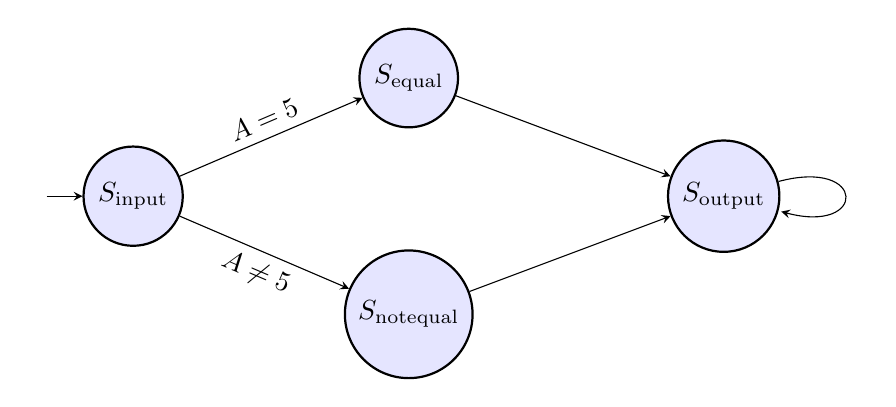
\begin{tikzpicture}[
    ->, >=stealth, auto, node distance=3.5cm,
    every state/.style={thick, fill=blue!10, minimum size=1.2cm},
    initial text=$ $
]

    \node[state, initial] (input) {$S_{\text{input}}$};
    \node[state, right of=input, yshift=1.5cm] (equal) {$S_{\text{equal}}$};
    \node[state, right of=input, yshift=-1.5cm] (notequal) {$S_{\text{notequal}}$};
    \node[state, right of=input, xshift=4cm] (output) {$S_{\text{output}}$};

    \path   (input) edge node [above, sloped] {$A=5$} (equal)
            (input) edge node [below, sloped] {$A \neq 5$} (notequal)
            (equal) edge node {} (output)
            (notequal) edge node {} (output)
            (output) edge [loop right] node {} (output);

\end{tikzpicture}

\end{document}
